% TODO:
% - 

%%%%%%%%%%%%%%%%%%%%%%%%%%%%%%%%%%%%%%%%%%%%%%%%%%%%
% documentclss
\documentclass[]{beamer}
%\documentclass[handout]{beamer} %Drucker Version
%\documentclass[draft]{beamer}


%%%%%%%%%%%%%%%%%%%%%%%%%%%%%%%%%%%%%%%%%%%%%%%%%%%%
% packages

\usepackage[utf8]{inputenc}
\usepackage[ngerman]{babel}
\usepackage[T1]{fontenc}

\usepackage{setspace}
\usepackage{ellipsis}
\usepackage{microtype}
\usepackage{lmodern}

\usepackage{lscape}
\usepackage{booktabs}			% \toprule, \midrule und \bottomrule in Tabellen
\usepackage{multirow}
\usepackage{paralist}

%\usepackage{scrhack} 
\usepackage{listings}
\lstset{
    language=C,
    breaklines=true,
    breakatwhitespace=true
    basicstyle=\footnotesize,
    numbers=left,
    numberstyle=\footnotesize,
    stepnumber=1,
    numbersep=5pt,
    extendedchars=true,
    inputencoding=utf8,
    breakindent=30pt,
    escapeinside={\%(}{\%)},
    captionpos=b
}

%\usepackage[pdftex]{graphicx} % Bereits von Beamer geladen
\graphicspath{{../Master_Thesis/images/}}
\usepackage{tikz}
\usepackage{wrapfig}
\usepackage{caption}         
\usepackage{subcaption}      
\usepackage{pgfgantt}        
\usepackage{rotating} 		

\hypersetup{
    pdftex,
    bookmarks, bookmarksopen, bookmarksopenlevel=1, bookmarksnumbered=true,
    pdfpagemode={UseNone},
    pdfpagelayout={SinglePage},
    plainpages=false,
    pdfkeywords={AUTOSAR, Virtualisierung, ECU, Python, CAN},
    pdfsubject={Virtualisierung von AUTOSAR Softwarekomponenten für die Erprobung},
    pdftitle={Virtualisierung von AUTOSAR Softwarekomponenten für die Erprobung},
    pdfauthor={Martin Wichmann},
}



\newcommand{\inputImage}[1]{\input{../Master_Thesis/images/#1}}
% Bild einfügen:
%\centering
%\resizebox{0.3\linewidth}{!}{\inputImage{autosar_overview.dia}}

\newtranslation[to=ngerman]{Example}{Beispiel}

\usetheme{Warsaw}

\AtBeginSubsection[]
{
   \begin{frame}
        \frametitle{Inhaltsübersicht}
        \tableofcontents[currentsection,hideallsubsections]
   \end{frame}
}



%%%%%%%%%%%%%%%%%%%%%%%%%%%%%%%%%%%%%%%%%%%%%%%%%%%%
% Title
\author{Martin Wichmann}
\title[Virtualisierung von AUTOSAR Softwarekomponenten]{Virtualisierung von AUTOSAR Softwarekomponenten für die Erprobung}
\subtitle{Kolloquium zur Masterarbeit}
\date{\today}
\institute{Ostfalia Hochschule für angewandte Wissenschaften}




%%%%%%%%%%%%%%%%%%%%%%%%%%%%%%%%%%%%%%%%%%%%%%%%%%%%
% begin document
\begin{document}

\begin{frame}
\maketitle
\end{frame}


\begin{frame}
\frametitle{Inhaltsübersicht}
\tableofcontents[hideallsubsections] % Einstellungen siehe Beamer User Guide Seite 99
\end{frame}





%%%%%%%%%%%%%%%%%%%%%%%%%%%%%%%%%%%%%%%%%%%%%%%%%%%%%%%%%%%%%%%%%%%5
% Einleitung
\section{Einleitung}
\label{sec:einleitung}

%%%%%
\begin{frame}
\frametitle{Einleitung}
    \begin{itemize}
        \item AUTOSAR mittlerweile etabliert
        \item Virtualisierung im Serverbereich üblich
        \item In dieser Arbeit:
        \begin{itemize}
            \item Evaluation von Virtualisierung im Embedded-Bereich
            \item Evaluation von AUTOSAR
        \end{itemize}
        \item Einsatzbereiche
        \begin{itemize}
            \item Lehre und Evaluation
            \item Reale Projekte
        \end{itemize}
        \item Schwerpunkt: Kommunikation und Virtualisierung
    \end{itemize}
\end{frame}


%%%%%%%%%%
%\subsection{Zielsystem}

%%%%%
\begin{frame}
\frametitle{Motivation}
    \begin{figure}[ht]
        \centering
        \resizebox{0.9\linewidth}{!}{\inputImage{arch_begin.dia}}
        \caption{Fallbeispiel}
        \label{fig:fallbeispiel}
    \end{figure}
\end{frame}



%%%%%%%%%%%%%%%%%%%%%%%%%%%%%%%%%%%%%%%%%%%%%%%%%%%%%%%%%%%%%%%%%%%5
% Grundlagen
\section{Grundlagen}
\label{sec:grundlagen}

%%%%%%%%%%
\subsection{Virtualisierung}
%%%%%
\begin{frame}
\frametitle{Überblick}
    \begin{itemize}
        \item Beschreibt eine Reihe von Techniken
        \item Ein reales System -> mehrere virtuelle Systeme
        \item Zentrales Element: Hypervisor
        \item Verschiedene Ziele:
        \begin{itemize}
            \item Zugriff auf verschiedene Betriebssysteme
            \item Wartbarkeit
            \item Skalierbarkeit
            \item Ausfallsicherheit
        \end{itemize}
    \end{itemize}
\end{frame}

%%%%%
\begin{frame}
\frametitle{Hypervisor Kategorien}
    \begin{figure}
        \centering
        \begin{subfigure}[b]{0.49\textwidth}
            \centering
            \resizebox{0.9\linewidth}{!}{\inputImage{virt_type1.dia}}
            \caption{Type 1-Hypervisor}
            \label{fig:hypervisor_type1}
        \end{subfigure}
        \begin{subfigure}[b]{0.49\textwidth}
            \centering
            \resizebox{0.9\linewidth}{!}{\inputImage{virt_type2.dia}}
            \caption{Type 2-Hypervisor}
            \label{fig:hypervisor_type2}
        \end{subfigure}
        \caption{Hypervisor Kategorien}
        \label{fig:hypervisor}
    \end{figure}
\end{frame}

%%%%%
\begin{frame}
\frametitle{Virtualisierung in eingebetteten Systemen}
    \begin{itemize}
        \item Auch bekannt als: Time and Space Partitioning
        \item SOCs immer Leistungsfähiger
        \item Automobil: ~50 Steuergeräte
        \item Spezielle Anforderungen
        \begin{itemize}
            \item Energieverbrauch
            \item Speichernutzung
            \item Sicherheit
            \item Determinismus und Echtzeitfähigkeit
        \end{itemize}
        \item Bereits im Einsatz: ARINC 653
    \end{itemize}
\end{frame}


%%%%%
\begin{frame}
\frametitle{ARINC 653 Übersicht}
    \begin{figure}[ht]
        \centering
        \resizebox{0.65\linewidth}{!}{\inputImage{arinc653.dia}}
        \caption{ARINC 653 Architektur Übersicht}
        \label{fig:arinc_653}
    \end{figure}
\end{frame}

%%%%%
\begin{frame}
\frametitle{Marktübersicht}
    \begin{itemize}
        \item PikeOS
        \item OKL4 Microvisor
        \item INTEGRITY Multivisor
        \item COQOS
        \item XtratuM
    \end{itemize}
\end{frame}

%%%%%
\begin{frame}
\frametitle{Vorteile und Nachteile}
    \begin{itemize}
        \item[$ + $] Unabhängigkeit vom Betriebssystem
        \item[$ + $] Sicherheit
        \item[$ + $] Wiederverwenden von altem Code
        \item[$ + $] IP-Schutz und Trennung von Software-Lizenzen
        \item[$ + $] Hypervisor klein und robust

        \item[$ - $] Single Point of Failure
        \item[$ - $] Leistungseinbußen
        \item[$ - $] Größere Folgen eines Ausfalls
    \end{itemize}
\end{frame}


%%%%%%%%%%
\subsection{AUTOSAR}

%%%%%
\begin{frame}
\frametitle{AUTOSAR Einleitung}
    \begin{itemize}
        \item AUTomotive Open System ARchitecture
        \item Systemarchitektur
        \item Entwicklungsmodell
        \item Entwickelt von und für Automobilindustrie
        \item "`Erbe"' von OSEK/VDX
        \item AUTOSAR ist nur Standard und beschreibt Schnittstellen
    \end{itemize}
\end{frame}

%%%%%
\begin{frame}[plain] % TODO: vielleicht plain da das Bild groß ist
%\begin{frame}
\frametitle{AUTOSAR Überblick}
    \begin{figure}[p]
        \centering
        \resizebox{0.6\linewidth}{!}{\inputImage{autosar_overview.dia}}
        \caption{Autosar Überblick}
        \label{fig:autosar_overview}
    \end{figure}
\end{frame}

%%%%%
\begin{frame}
\frametitle{Grundkonzepte}
    \begin{itemize}
        \item Systembeschreibung (System Description)
        \item Kommunikations-Informationen
        \item Quellcode und Objektdateien
        \item AUTOSAR Entwicklungswerkzeug
        \begin{itemize}
            \item Basis-Software-Implementation
            \item Basis-Software-Konfigurator
            \item Runtime-Enviroment-Generator
        \end{itemize}
    \end{itemize}
\end{frame}

%%%%%
\begin{frame}
\frametitle{Entwicklungsprozess}
    \begin{figure}[ht]
        \centering
        \resizebox{\linewidth}{!}{\inputImage{Autosar_Prozess.dia}}
        \caption{AUTOSAR-Entwicklungsprozess}
        \label{fig:autosar_prozess}
    \end{figure}
\end{frame}

% TODO: RTE, VFB, BSW

%%%%%
\begin{frame}
\frametitle{TODO}
    \begin{figure}[ht]
        \centering
        \resizebox{\linewidth}{!}{\inputImage{autosar_layer.dia}}
        \caption{AUTOSAR-Schichtenmodell}
        \label{fig:autosar_layer}
    \end{figure}
\end{frame}

%%%%%
\begin{frame}
\frametitle{TODO}
    \begin{figure}[ht]
        \centering
        \resizebox{\linewidth}{!}{\inputImage{autosar_refined_layer.dia}}
        \caption{AUTOSAR-Schichtenmodell mit genauerer Aufteilung}
        \label{fig:autosar_refined_layer}
    \end{figure}
\end{frame}

%%%%%
\begin{frame}
\frametitle{Kritik an AUTOSAR}
    \begin{itemize}
        \item Effizienz
        \item Umfang des Standards
        \item Schnelle Entwicklung von AUTOSAR
        \item Bindung an Hersteller
        \item Starke Relevanz der Designphase
        \item Dokumentation der Konfiguration
        \item Portabilität von Softwarekomponenten
    \end{itemize}
\end{frame}




%%%%%%%%%%
\subsection{Netzwerkmanagment}
%%%%%
\begin{frame}
\frametitle{TODO}

\end{frame}




%%%%%%%%%%
\subsection{Funktionale Sicherheit}
%%%%%
\begin{frame}
\frametitle{TODO}
    \begin{figure}[!htbp]
        \center
        \inputImage{ISO_26262_Lifecycle.dia}
        \caption{Sicherheitslebenszyklus nach ISO 26262}
        \label{fig:lifecycle}
    \end{figure}
\end{frame}







%%%%%%%%%%%%%%%%%%%%%%%%%%%%%%%%%%%%%%%%%%%%%%%%%%%%%%%%%%%%%%%%%%%5
% Umsetzung
\section{Umsetzung}
\label{sec:umsetzung}

%%%%%
\begin{frame}
\frametitle{Überblick}
    \begin{figure}[ht]
        \centering
        \inputImage{arch_finished.dia}
        \caption{Vollständige Architektur}
        \label{fig:arch_finished}
    \end{figure}
\end{frame}




%%%%%%%%%%
\subsection{Virtualisierung}
%%%%%
\begin{frame}
\frametitle{TODO}

\end{frame}




%%%%%%%%%%
\subsection{Kommunikation Linux und AUTOSAR}
%%%%%
\begin{frame}
\frametitle{TODO}

\end{frame}




%%%%%%%%%%
\subsection{Kommunikation AUTOSAR und Scheinwerfer-ECU}
%%%%%
\begin{frame}
\frametitle{TODO}

\end{frame}




%%%%%%%%%%
\subsection{Entwicklung AUTOSAR Komponente}
%%%%%
\begin{frame}
\frametitle{TODO}
    \begin{figure}[ht]
        \centering
        \resizebox{\linewidth}{!}{\inputImage{SMLS_Modell.dia}}
        \caption{Entwickeltes AUTOSAR Modell}
        \label{fig:smls_modell}
    \end{figure}
\end{frame}




%%%%%%%%%%
\subsection{Entwicklung steuernde Komponente}
%%%%%
\begin{frame}
\frametitle{TODO}
    \begin{figure}
        \centering
        \begin{subfigure}[b]{0.59\textwidth}
            \centering
            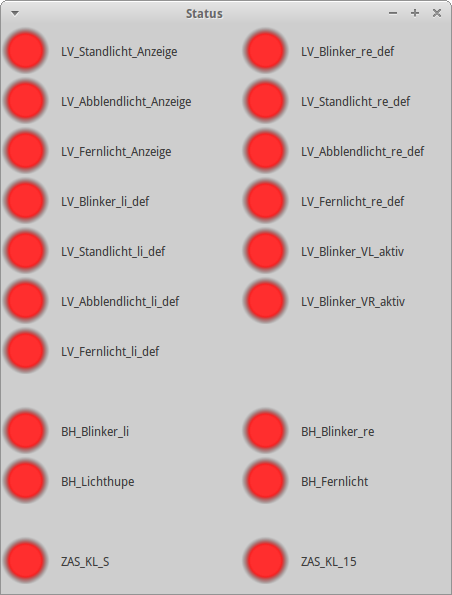
\includegraphics[width=\textwidth]{vcan_app_status}
            \caption{Status-Fenster}
            \label{fig:vcan_app_status}
        \end{subfigure}
        \begin{subfigure}[b]{0.39\textwidth}
            \centering
            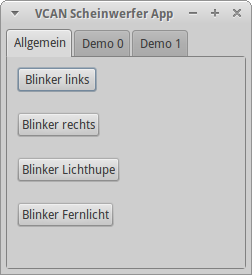
\includegraphics[width=\textwidth]{vcan_app_control}
            \caption{Kontroll-Fenster}
            \label{fig:vcan_app_control}
        \end{subfigure}
        \caption{Oberfläche der VCAN-Applikation}
        \label{fig:vcan_app}
    \end{figure}
\end{frame}





%%%%%%%%%%%%%%%%%%%%%%%%%%%%%%%%%%%%%%%%%%%%%%%%%%%%%%%%%%%%%%%%%%%5
% Fazit
\section{Analyse und Fazit}
\label{sec:analyse_fazit}

%%%%%%%%%%
\subsection{Analyse}
%%%%%
\begin{frame}
\frametitle{TODO}
    \begin{figure}
        \centering
        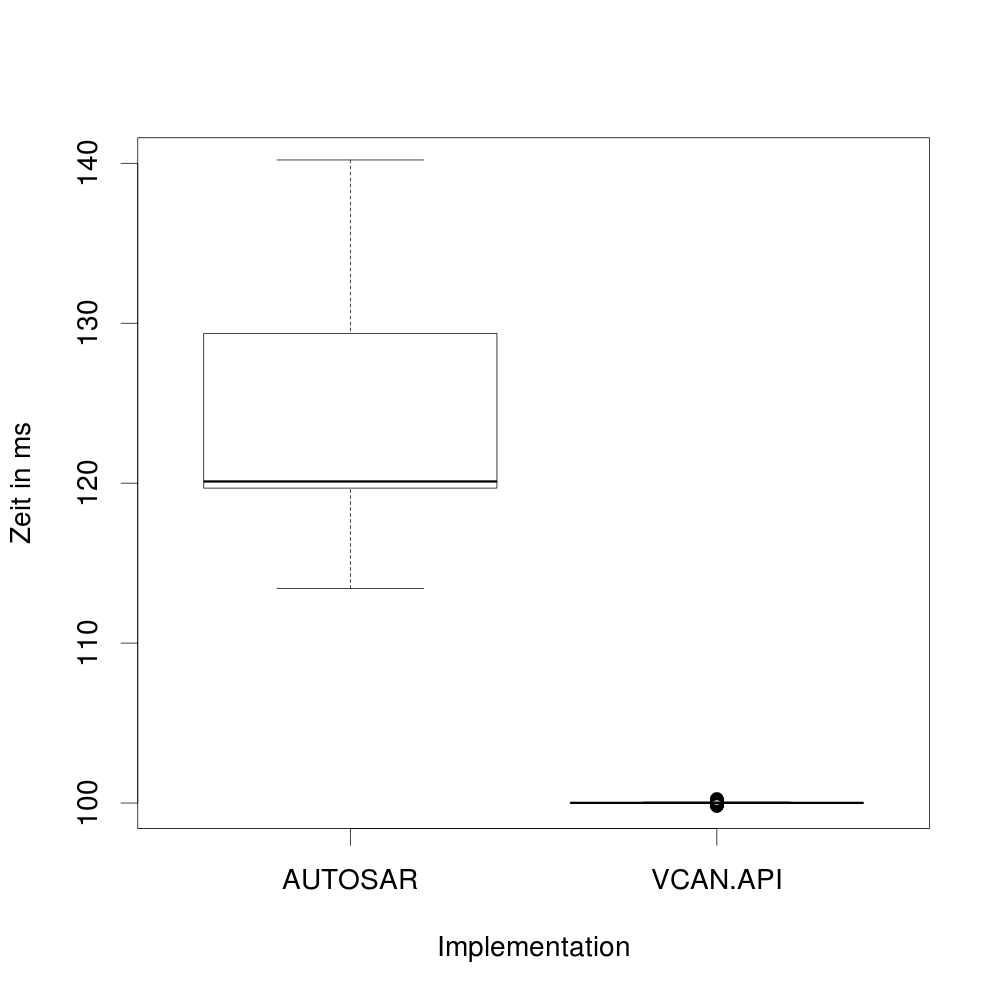
\includegraphics[width=0.5\textwidth]{boxplot}
        \caption[Zeitanalyse des VCAN als Boxplots]{Zeitanalyse des VCAN als Boxplots}
        \label{fig:timinganalyse}
    \end{figure}
\end{frame}



%%%%%%%%%%
\subsection{Fazit und Ausblick}
%%%%%
\begin{frame}
\frametitle{Fazit}

\end{frame}


%%%%%
\begin{frame}
\frametitle{Ausblick}

\end{frame}










%%%%%%%%%%%%%%%%%%%%%%%%%%%%%%%%%%%%%%%%%%%%%%%%%%%%%%%%%%%%%%%%%%%5
% Literaturangaben
\appendix
\section*{Literatur}
\label{sec:Literatur}

\begin{frame}


\begin{thebibliography}{10}

\bibitem[1]{1} \textsc{Olaf Kindel, Mario Driedrich}: {\em Softwareentwicklung mit AUTOSAR: Grundlagen, Engineering, Management in der Praxis.} dpunkt.verlag, 2009.

\bibitem[2]{2} \textsc{Peter Löw, Roland Pabst, Erwin Petry}: {\em Funktionale Sicherheit in der Praxis.} dpunkt.verlag, 2010.

\bibitem[3]{3} \textsc{AUTOSAR}: {\em Technical Overview.} Online unter: \url{http://autosar.org/download/R3.1/AUTOSAR_TechnicalOverview.pdf}

\bibitem[4]{4} \textsc{AUTOSAR}: {\em Layered Software Architecture.} Online unter: \url{http://autosar.org/download/R3.1/AUTOSAR_LayeredSoftwareArchitecture.pdf}

\end{thebibliography}


\end{frame}

\end{document}

